\chapter{Lecture 17 - Generating and Plotting Fourier Series in MATLAB}
\label{ch:lec17}
\section{Objectives}
\begin{itemize}
\item Demonstrate how to carry out Fourier series expansions using MATLAB.
\item Give a qualitative demonstration of convergence behavior of Fourier series.
\item Demonstrate Cosine and Sine series expansions.
\end{itemize}
In this lecture, we will illustrate the process of Fourier series expansions with three examples.

\vspace{0.5cm}

\noindent\textbf{Example \#1:}
Carry out the Fourier series expansion of the function given in Equation \ref{eq:lec17-ex1}, illustrated in Figure \ref{fig:lec17-ex1-fx}:
\begin{equation}
f(x) = 
\begin{cases}
0, & -\pi \le x < 0 \\
\pi - x, & 0 \le x \le \pi
\end{cases}
\label{eq:lec17-ex1}
\end{equation}
\begin{marginfigure}
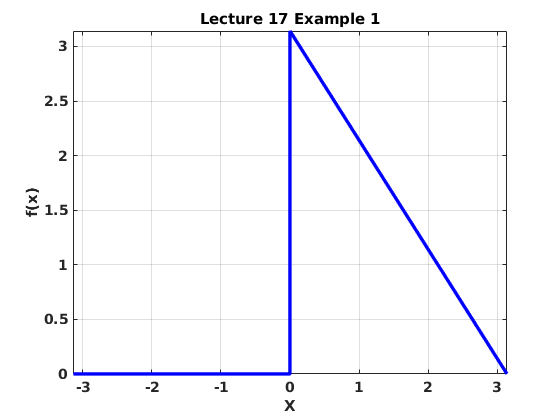
\includegraphics{lec17_ex1_fx.png}
\caption{Example \#1 $f(x)$.}
\label{fig:lec17-ex1-fx}
\end{marginfigure}
We wish to represent this function as:
\begin{equation*}
f(x) = \frac{a_0}{2} + \sum\limits_{n=1}^{\infty} \left[a_n \cos{\frac{n \pi x}{p}} + b_n \sin{\frac{n \pi x}{p}} \right]
\end{equation*}
where, in this case, $p = \pi$.  Even though we are only interested in the function in the interval $[-\pi, \pi]$, since the Fourier series represents the function in terms of a constant and an infinite linear combination of of periodic functions, we should think of the function that we are representing as periodic.\sidenote{This outlook will help us understand the convergence behavior of the Fourier series; especially at the boundaries.}

We have everything we need; it is just a matter of calculating the coefficients from Equation \ref{eq:Fourier-Coeff}.  Rather than carrying out the calculations with pencil and paper we will use MATLAB.  In the listing below we will step through the code necessary to calculate Fourier coefficients through \lstinline{N=5}.

\begin{lstlisting}[name=lec17-ex1,style=myMatlab]
clear
clc
close 'all'

N = 5; % specify number of coefficients

f = @(x) ex1(x); 
p = pi; % specifiy period
\end{lstlisting}
We start, as always, by clearing out the workspace memory and command-prompt output and closing any open figures.  We also need to represent $f(x)$ in MATLAB; we will do this with a local function named \lstinline{ex1(x)}.\sidenote{Since inline functions must appear \emph{after} all of the other code in a MATLAB script file, the code for \lstinline{ex1(x)} will be presented last.}  

The integrals needed to determine the Fourier coefficients will be evaluated numerically with the MATLAB built-in function \lstinline{integral()}.\sidenote{This function has default signature \lstinline{Q = integral(FUN,A,B)} and it approximates the integral of function \lstinline{FUN} over the interval \lstinline{A} to \lstinline{B} using global adaptive quadrature.  The error tolerances for this numeric integration algorithm can be specified by the user; in most cases we will use default values.  There are several standard algorithms for numerically computing integrals---called quadrature---that the interested student can read about in the numerical methods portion of this text.} Let us start with $a_0$ which, as a reminder, is computed by:
\begin{equation*}
a_0 = \frac{1}{p}\int_{-p}^{p} f(x) \ dx
\end{equation*}

\begin{lstlisting}[name=lec17-ex1,style=myMatlab]
a0 = (1/p)*integral(f,-p,p);
FF = @(x) a0/2;
\end{lstlisting}
The first line of the listing numerically evaluates $a_0$; the second line creates an anonymous function and initializes it to the first term in the Fourier expansion.

We will use a loop to construct the remaining terms in the Fourier expansion.\marginnote{Recall:
\begin{align*}
an &= \frac{1}{p}\int_{-p}^p f(x) \cos{\frac{n \pi x}{p}}\ dx \\
bn &= \frac{1}{p}\int_{-p}^p f(x) \sin{\frac{n \pi x}{p}}\ dx
\end{align*}
Note how you can practically read the equation directly from the MATLAB code.
}
\begin{lstlisting}[name=lec17-ex1,style=myMatlab]
for n = 1:N
    an = (1/p)*integral(@(x) f(x).*cos(n*pi*x/p),-p,p);
    bn = (1/p)*integral(@(x) f(x).*sin(n*pi*x/p),-p,p);
    FF = @(x) FF(x) + an*cos(n*pi*x/p) + bn*sin(n*pi*x/p); 
end
\end{lstlisting}
Note in the last line where we append the newly computed terms to the Fourier series expansion \lstinline{FF(x)}.  Now we have a function, $\lstinline{FF(x)}$, that represents the Fourier series expansion with $N=5$ terms.  In the next listing we add the code to plot the function and verify that it makes sense.
\marginnote{

\vspace{2.25cm}

Referring to the annotations:



\noindent \ref{lst:annotation1} Using \lstinline[style=myMatlab]{sprintf()} allows us to combine the variable \lstinline{n} in the title string.  

\vspace{0.25cm}

\noindent \ref{lst:annotation2} Optional name-value pairs such as \lstinline{'Linewidth',3}, \lstinline{'FontSize',16}, and \lstinline{'FontWeight','bold'} help make the plot and labels more readable.



}

\begin{lstlisting}[name=lec17-ex1,style=myMatlab]
Nx = 1000;
X = linspace(-p,p,Nx);

plot(X,f(X),'-b',...
    X,FF(X),'--r',...
    'LineWidth',3)
title_str = sprintf('Example 1, n = %d',n);/*!\annotation{lst:annotation1}!*/
title(title_str,'FontSize',16,...
    'FontWeight','bold');
xlabel('X','FontSize',14,... /*!\annotation{lst:annotation2}!*/
    'FontWeight','bold');
ylabel('f(X)','FontSize',14,...
    'FontWeight','bold');
grid on
legend('f(x)','FF(x)')/*!\annotation{lst:annotation3}!*/
set(gca,'FontSize',12,...
    'FontWeight','bold');/*!\annotation{lst:annotation4}!*/
\end{lstlisting} \marginnote[-2.5cm]{
\vspace{0.25cm}

\noindent \ref{lst:annotation3} Make a habit of using legends for graphs that include multiple data series. Once again, this makes the plot more readable.

\vspace{0.25cm}

\noindent \ref{lst:annotation4} The argument \lstinline[style=myMatlab]{gca} means ``get current axis.''  Calling the \lstinline[style=myMatlab]{set()} function with name-value pairs \lstinline{'FontSize',10} and \lstinline{'FontSize','bold'} sets the font size and weight for the axis markings.

\vspace{0.25cm}

\noindent In general it is important that your plots look good.

}



 \setcounter{lstannotation}{0}
The resulting Fourier series expansion is shown in Figure \ref{fig:lec17-ex1-n5}. If we want to increase the number of Fourier series terms in the expansion, we need only change \lstinline{N}.  Figure \ref{fig:lec17-ex1-n15} shows the series expansion with \lstinline{N=15} terms.
\begin{marginfigure}
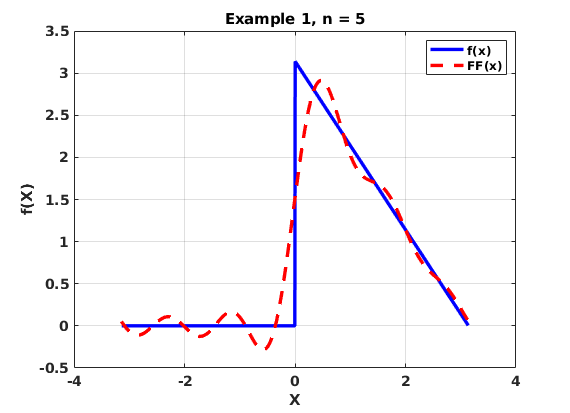
\includegraphics{lec17_ex1_n5.png}
\caption{Fourier series expansion with \lstinline{N=5}.}
\label{fig:lec17-ex1-n5}
\end{marginfigure}

\begin{marginfigure}
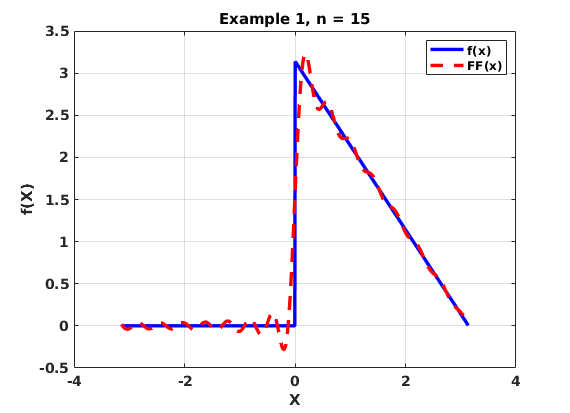
\includegraphics{lec17_ex1_n15.png}
\caption{Fourier series expansion with \lstinline{N=15}.}
\label{fig:lec17-ex1-n15}
\end{marginfigure} 
Some things to note about the resulting Fourier series representation of \lstinline{f(x)}:
\begin{enumerate}
\item As \lstinline{n} increases, \lstinline{FF(x)} generally ``looks more like'' \lstinline{f(x)}.  
\item At the discontinuity in \lstinline{f(x)}, the Fourier series representation appears to be converging on the midpoint between $f(x^-)$ and $f(x^+)$ as the theory says it should.
\item The Fourier series representation near the point of discontinuity has ``wiggliness'' that doesn't go away as \lstinline{n} increases.
\item In particular, note the undershoot and overshoot of $f(x)$ to the left and right respectively of $f(0)$.  This is called ``Gibbs phenomena'' and it does not go away as \lstinline{n} increases but it moves closer to the point of discontinuity.  
\end{enumerate}
As Figure \ref{fig:lec17-ex1-n150} shows, as \lstinline{N} is increased, we can make \lstinline{FF(x)} arbitrarily close to \lstinline{f(x)} with the exception of the perturbations at the point of discontinuity.
\begin{marginfigure}
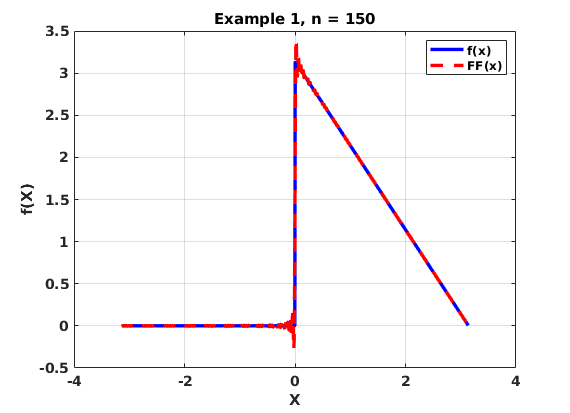
\includegraphics{lec17_ex1_n150.png}
\caption{Fourier series expansion with \lstinline{N=150}.}
\label{fig:lec17-ex1-n150}
\end{marginfigure}

\newthought{An important matter} that we have not yet dealt with is how to represent piece-wise continuous functions like $f(x)$ in MATLAB.\sidenote{For whatever reason, piece-wise continuous functions are intensively used in \emph{textbooks} on partial differential equations---I am not so sure that they are as important in real-life applications.}  As stated previously, we will use a \emph{local function} to do this.  The code is shown in the listing below.

\begin{lstlisting}[name=lec17-ex1,style=myMatlab]
%% Local functions 
function y = ex1(x) 
[m,n] = size(x); /*!\annotation{lst:annotation1-1}!*/
y = nan(m,n); /*!\annotation{lst:annotation1-2}!*/
for i = 1:length(x) /*!\annotation{lst:annotation1-3}!*/
    if (x(i) >= -pi) && (x(i) < 0) 
        y(i) = 0;
    elseif (x(i) >= 0) && (x(i) <= pi) /*!\annotation{lst:annotation1-4}!*/
        y(i) = pi - x(i);
    end
end
end
\end{lstlisting} \setcounter{lstannotation}{0}
Some notes on the annotations for this listing:

\vspace{0.25cm}

\noindent \ref{lst:annotation1-1}  We use the MATLAB built-in function \lstinline[style=myMatlab]{size()} to get the dimensions of the input vector.  The return values \lstinline{[m,n]} give the number of rows and columns of \lstinline{x} respectively. For this function we are implicitly expecting \lstinline{x} to be a vector, but it can be either a row-vector or a column vector.

\vspace{0.25cm}

\noindent \ref{lst:annotation1-2} We construct the output vector \lstinline{y} using the \lstinline{nan()} function.  This line makes the vector \lstinline{y} the same size and shape as the input vector \lstinline{x}.  


\vspace{0.25cm}

\noindent \ref{lst:annotation1-3} We use the built-in function \lstinline[style=myMatlab]{length()} to get the number of elements of \lstinline{x}.  This is a bit of a hack since, if \lstinline{x} were \textbf{\emph{not}} a vector, \lstinline{ex1(x)} would no longer work properly.\sidenote[][-5.0cm]{It would be a good idea to verify that the input \lstinline{x} is actually a vector.  MATLAB, like most other languages, includes features to enforce assumptions like this. The code: \lstinline[style=myMatlab]{assert(min(size(x))==1,'x must be a vector')} would raise an error in MATLAB if the minimum dimension of \lstinline{x} is anything other than 1.  That would be one way to ensure \lstinline{x} is a vector.}

\vspace{0.25cm}

\noindent \ref{lst:annotation1-4} The symbol \lstinline{&&} is ``element-wise and.''  Pay attention to use of \lstinline{>=} and \lstinline{<=} operators to get the details of the intended function correct.

\vspace{0.5cm}

\noindent\textbf{Example \#2:}  Carry out the Fourier series expansion of the function given in Equation \ref{eq:lec17-ex2}, illustrated in Figure \ref{fig:lec17-ex2-fx}.
\begin{equation}
f(x) = 
\begin{cases}
-1, & -\pi \le x < 0 \\
1, & 0 \le x \le \pi
\end{cases}
\label{eq:lec17-ex2}
\end{equation}
\begin{marginfigure}[-6.0cm]
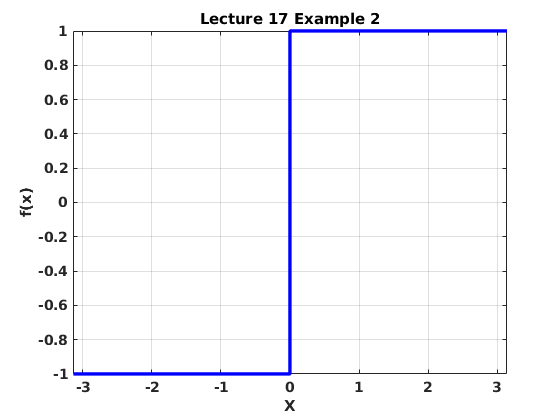
\includegraphics{lec17_ex2_fx.png}
\caption{Example \#2 $f(x)$.}
\label{fig:lec17-ex2-fx}
\end{marginfigure}
Fourier series expansions of this function are shown in Figures \ref{fig:lec17-ex2-n5} through \ref{fig:lec17-ex2-n150}.
\begin{marginfigure}[-1.0cm]
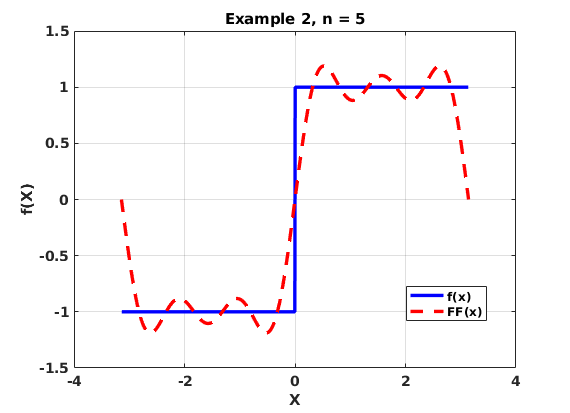
\includegraphics{lec17_ex2_n5.png}
\caption{Fourier series expansion with \lstinline{N=5}.}
\label{fig:lec17-ex2-n5}
\end{marginfigure}

\begin{marginfigure}
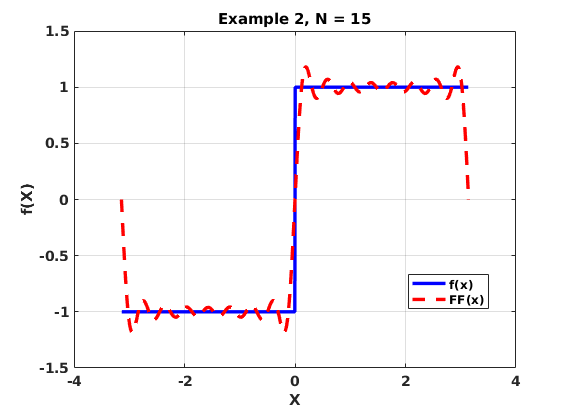
\includegraphics{lec17_ex2_n15.png}
\caption{Fourier series expansion with \lstinline{N=15}.}
\label{fig:lec17-ex2-n15}
\end{marginfigure}

\begin{marginfigure}
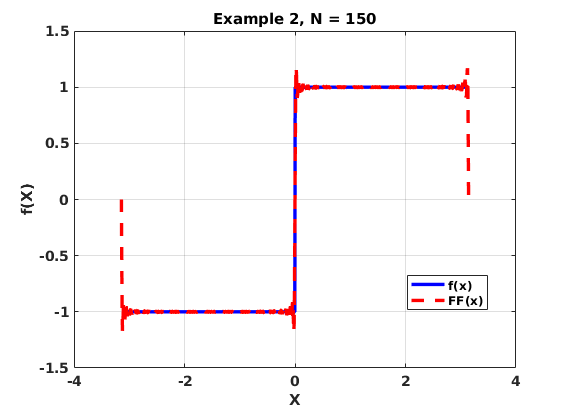
\includegraphics{lec17_ex2_n150.png}
\caption{Fourier series expansion with \lstinline{N=150}.}
\label{fig:lec17-ex2-n150}
\end{marginfigure}
Some notes:
\begin{enumerate}
\item As with the first example, the function has the Gibbs phenomena near the discontinuity at $x=0$.  
\item Also, as with the first example, the Gibbs phenomena does not go away as $N$ increases, but it gets more ``peaked'' and closer to the origin.
\item Unlike the first example, we get the Gibbs phenomena and wiggliness at the ends also.  This is because the Fourier series representation is periodic; the periodic extension of this function has discontinuities at the endpoints since $f(-\pi) \ne f(\pi)$.  
\item You should also note that this function is \emph{even}.  That means we expect $a_0$ and all values of $a_n$ to be equal to zero. If we modify the for-loop to output values for the $a_n$ coefficients we get all zeros.

\begin{lstlisting}[style=myMatlab]
for n = 1:N
    an = (1/p)*integral(@(x) f(x).*cos(n*pi*x/p),-p,p);
    fprintf('a_%d = %g \n',n,an);
    bn = (1/p)*integral(@(x) f(x).*sin(n*pi*x/p),-p,p);
    FF = @(x) FF(x) + an*cos(n*pi*x/p) + bn*sin(n*pi*x/p); 
end
\end{lstlisting}
\end{enumerate}

%\begin{marginfigure}
%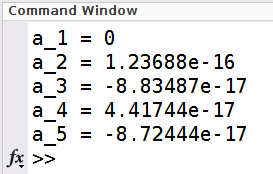
\includegraphics{lec17_ex2_an.png}
%\end{marginfigure}

\vspace{5.0cm}

\noindent\textbf{Example \#3:} Construct the Fourier series expansion of the function given in Equation \ref{eq:lec17-ex3-fx}.

\begin{equation}
f(x) = x^2, \ \ x \in[0,2]
\label{eq:lec17-ex3-fx}
\end{equation}

This function is not periodic and, unlike the previous examples, does not even span a symmetric interval about the origin.  In this case we will still use the same Fourier series formulas but we will construct a ``reflection'' about the origin.  This reflection can be \emph{even-}, \emph{odd-}, or it can be an \emph{identity-reflection} with respect to the y-axis; these correspond to the Cosine expansion, Sine expansion and the full Fourier series expansions.  These different expansion options are shown in Figure \ref{fig:lec17-ex3}.

\begin{figure}
\subfloat[]{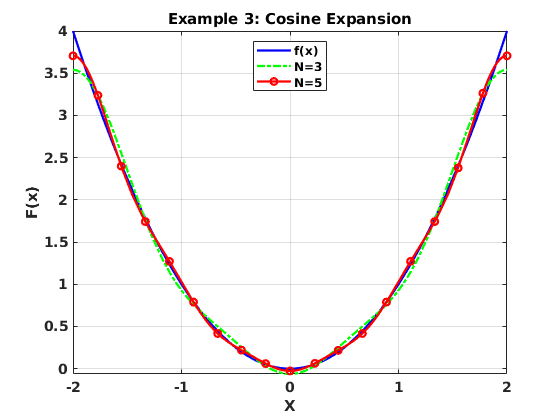
\includegraphics[width=2in]{lec17_ex3_cos.png}}
\subfloat[]{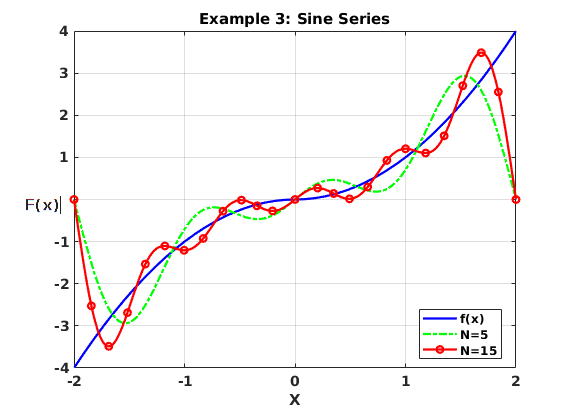
\includegraphics[width=2in]{lec17_ex3_sin.png}} \\
\begin{center}
\subfloat[]{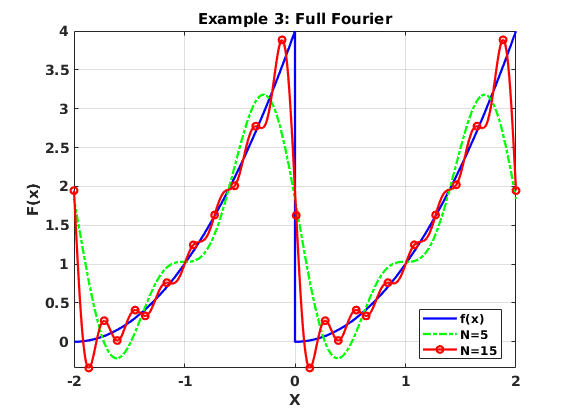
\includegraphics[width=2in]{lec17_ex3_full.png}}
\end{center}
\label{fig:lec17-ex3}
\caption{Even-, odd- and identity-reflection for $f(x)=x^2$.}
\end{figure}

Note that the convergence behavior for the Fourier expansion is different for each case.\marginnote{As you can see, in cases where you can choose which expansion you use, some choices are good and some are bad.  As we will see in coming chapters, we often do not have a choice in which set of orthogonal functions we will use to do our expansion so, sadly, we cannot pick one that we think will be best.  What we \emph{can} do is analyze the expansion that we \emph{do} get and understand the convergence behavior by examining the continuity of the functions and derivatives of functions that we are representing.}
\begin{itemize}
\item For the even-reflection Cosine expansion convergence is very rapid.  Both $f(x)$ and $f^{\prime}(x)$ are continuous throughout the interval $x\in (-2,2)$.  The function itself is continuous at the end-points but notice that the derivative is not.  If you were to draw an additional period on the left and right-hand side of the cosine expansion, $f^{\prime}(x)$ would have a discontinuity; that explains the (relatively) poor convergence of the series at the end-points.
\item For the odd-reflection Sine expansion the function and derivative is continuous throughout the domain.  The derivative of the function is continuous at the periodic end-points but $f(x)$ itself is not.  This explains why the Sine series expansion converges to zero at both end-points.  
\item The identity-reflection full Fourier series has discontinuities in $f(x)$ and $f^{\prime}(x)$ at both endpoints and at $x=0$.  The convergence behavior is correspondingly bad.
\end{itemize}
